% bookformat.tex — 170 x 240 mm book layout + 3 mm bleed (176 x 246 mm paper),
% a common format for printed PhD theses. To change the trim size, edit \geometry
% and the TrimBox/BleedBox values below (in bp; 1 mm = 2.8346 bp).
% Load it after preamble.tex and thesisinfo.tex.
% BLEED VERSION: 3 mm bleed on every side. The paper is 176 x 246 mm; the final
% trimmed page (170 x 240 mm) sits centred, so all margins are 3 mm larger.
\geometry{papersize={176mm,246mm}, inner=23mm, outer=23mm,
	top=28mm, bottom=19mm, includefoot=false,
	headheight=12pt, headsep=11mm, footskip=0pt}

% Fonts (all SIL Open Font License): body text in Libertinus Serif 10.5 pt on 14 pt,
% equations in Libertinus Math, headings, running heads, tabs and captions labels in Carlito.
\usepackage{pdfpages}
\pdfpageattr{/TrimBox [8.504 8.504 490.394 688.819] /BleedBox [0 0 498.898 697.323]}
\usepackage{libertinus}% Libertinus Serif (text)
\usepackage[lining]{carlito}% Carlito (sans: headings, running heads, tabs)
\usepackage{libertinust1math}% Libertinus Math (equations)
\renewcommand*{\familydefault}{\rmdefault}\normalfont
\setlength{\emergencystretch}{2em}% lets TeX loosen a line slightly instead of overrunning the margin
\setlength{\intextsep}{10pt}% space above and below [H] figures
\makeatletter\g@addto@macro\@floatboxreset{\def\@tempa{table}\ifx\@captype\@tempa\small\fi}\makeatother% tables one size smaller than the text
\renewcommand{\textsc}[1]{#1}% the class maps \textsc to a weight Libertinus lacks; print the text as written
\renewcommand{\normalsize}{\fontsize{10.5}{14}\selectfont}
\singlespacing\normalsize
\setlength{\parindent}{0pt}
\setlength{\parskip}{14pt}

% Headings
\definecolor{chaptertan}{cmyk}{0,0.30,0.60,0.21}
\definecolor{abstractgrey}{RGB}{220,221,222}% background of the abstract pages
\titleformat{\section}{\sffamily\fontsize{12}{14}\bfseries\color{black}}{\thesection}{0.5em}{}
\titleformat{\subsection}{\sffamily\fontsize{11}{14}\bfseries\color{black}}{\thesubsection}{0.5em}{}
\titleformat{\subsubsection}{\sffamily\fontsize{11}{14}\bfseries\itshape}{}{0pt}{}
\titlespacing*{\section}{0pt}{14pt}{-14pt}
\titlespacing*{\subsection}{0pt}{0pt}{-14pt}
\titlespacing*{\subsubsection}{0pt}{0pt}{-14pt}

% Chapter opener on its own right-hand page, with the "This chapter is based on" note
\definecolor{basedonrule}{cmyk}{0.77,0.37,0.30,0}
\newcommand{\printbasedon}{%
  \ifx\basedontext\empty\else
    \par\vspace{42mm}%
    \noindent\begin{minipage}{\textwidth}\setlength{\parskip}{0pt}%
      {\color{basedonrule}\rule{\textwidth}{1.5pt}}\par\vspace{3pt}%
      \sffamily\fontsize{9.5}{14}\selectfont\raggedleft
      {\bfseries\basedonhead}\par
      \mdseries\basedontext
    \end{minipage}%
    \gdef\basedontext{}%
  \fi}
\titleformat{\chapter}[display]
  {\thispagestyle{empty}\raggedleft\sffamily}
  {\fontsize{54}{60}\bfseries\color{chaptertan}\chaptertitlename~\thechapter}
  {8mm}{\fontsize{14}{18}\bfseries\color{black}}[\printbasedon\clearpage]

% In the book the author block is dropped and the abstract sits on a grey page
\renewcommand{\chapterauthors}[1]{}
\renewenvironment{chapterabstract}[1][Abstract]
  {\clearpage\ifodd\value{page}\thispagestyle{empty}\null\clearpage\fi% reach a left-hand page
   \pagecolor{abstractgrey}\thispagestyle{empty}\null\clearpage% grey left page facing the abstract
   \thispagestyle{empty}\enlargethispage{2\baselineskip}%
   \if\relax\detokenize{#1}\relax\vspace*{0pt}\else\section*{#1}\vspace{14pt}\fi\setlength{\parskip}{6pt}\fontsize{10}{13.5}\selectfont}% abstracts slightly smaller so each fits on one page
  {\par\clearpage\nopagecolor\cleardoublepage}

% Unnumbered chapters (Acknowledgements, Prologue, appendices): title at the top, text follows
\titleformat{name=\chapter,numberless}[block]
  {\raggedright\sffamily\fontsize{14}{18}\bfseries\color{black}}{}{0pt}{}
\titlespacing*{\chapter}{0pt}{45mm}{0pt}
\titlespacing*{name=\chapter,numberless}{0pt}{-8mm}{4pt}

% Running heads at the top, grey: "30 | Chapter 1" (left pages), "Short title | 31" (right pages)
\setlength{\headwidth}{\textwidth}
\fancyhf{}
\renewcommand{\headrulewidth}{0pt}
% \shortchaptertitle (the right-hand running head) is defined in thesisinfo.tex
\newcommand{\evenheadtext}{\ifnum\value{chapter}>0 Chapter~\thechapter\fi}
\newcommand{\oddheadtext}{\shortchaptertitle}
\fancyhead[LE]{\sffamily\color{gray}{\fontsize{9}{9}\selectfont\thepage}%
  \hspace{0.5em}\textbar\hspace{0.5em}{\fontsize{8}{9}\selectfont\evenheadtext}}
\fancyhead[RO]{\sffamily\color{gray}{\fontsize{8}{9}\selectfont\oddheadtext}%
  \hspace{0.5em}\textbar\hspace{0.5em}{\fontsize{9}{9}\selectfont\thepage}}
\fancypagestyle{plain}{\fancyhf{}\renewcommand{\headrulewidth}{0pt}}
\let\oldappendix\appendix
\renewcommand{\appendix}{\oldappendix
  \renewcommand{\evenheadtext}{Appendices}\renewcommand{\oddheadtext}{Appendices}%
  % appendix headings: larger, with a blank line before the text
  \titleformat{\section}{\sffamily\fontsize{14}{18}\bfseries\color{black}}{\thesection}{0.5em}{}%
  \titlespacing*{\section}{0pt}{0pt}{0pt}%
  \titleformat{\subsection}{\sffamily\fontsize{11}{14}\bfseries\color{black}}{\thesubsection}{0.5em}{}%
  \titlespacing*{\subsection}{0pt}{0pt}{-6pt}}

% Contents heading in the same style as other front-matter headings
\renewcommand{\cfttoctitlefont}{\sffamily\fontsize{14}{18}\selectfont\bfseries\color{black}}

% Captions and bibliography
\captionsetup{font={small,color=black}, labelfont={bf,sf}, labelsep=period, width=\textwidth}
\renewcommand{\bibfont}{\fontsize{8}{10.5}\selectfont}
% URLs in the text font
\urlstyle{same}

% Chapter thumb tabs on right-hand pages (tan tab at the page edge, stepping down per chapter).
% Each tab is 16.3 mm tall, so about 12 tabs (chapters + appendix) fit down the page edge.
\newcommand{\thumblabel}{\arabic{chapter}}
\newcommand{\thumbindex}{\value{chapter}}
\newif\ifthumbtab
\newcommand{\thumbtab}{%
  \ifnum\value{chapter}>0 \thumbtabtrue\fi
  \ifthumbtab
  \begin{tikzpicture}[remember picture,overlay]
    \pgfmathsetlengthmacro{\thumbtop}{-24.9mm-16.3mm*(\thumbindex-1)}
    \fill[chaptertan,rounded corners=1.2mm]
      ([xshift=-16.7mm,yshift=\thumbtop-3mm]current page.north east) rectangle ++(17mm,-16.3mm);% 13.7 mm visible after trimming
    \node[text=white,font=\sffamily\fontsize{12}{12}\selectfont\bfseries]
      at ([xshift=-11.35mm,yshift=\thumbtop-11.15mm]current page.north east) {\thumblabel};
  \end{tikzpicture}%
  \fi}
\fancyhead[RO]{\thumbtab\sffamily\color{gray}{\fontsize{8}{9}\selectfont\oddheadtext}%
  \hspace{0.5em}\textbar\hspace{0.5em}{\fontsize{9}{9}\selectfont\thepage}}
\let\oldappendixthumb\appendix
\renewcommand{\appendix}{% the appendix tab sits one step below the last chapter's tab
  \edef\thumbindex{\the\numexpr\value{chapter}+1\relax}\oldappendixthumb
  \thumbtabtrue\renewcommand{\thumblabel}{A}}

% No running head or tab on blank left-hand pages before a chapter opener
\usepackage{emptypage}

% Paragraph headings (e.g. "Perturbation waveforms."): black italic on their own line, as in the proof
\titleformat{\paragraph}[block]{\fontsize{11}{14}\itshape\color{black}}{}{0pt}{}
\titlespacing*{\paragraph}{0pt}{0pt}{-14pt}
\titleformat{\subparagraph}[block]{\fontsize{10.5}{14}\itshape\color{black}}{}{0pt}{}
\titlespacing*{\subparagraph}{0pt}{0pt}{-14pt}

% Black list markers, numbers and contents entries (the class sets them in red)
\renewcommand*\labelitemi{\textbullet}
\renewcommand*\labelitemii{--}
\renewcommand*\labelitemiii{$\diamond$}
\renewcommand*\labelitemiv{\textperiodcentered}
\renewcommand{\labelenumi}{\arabic{enumi}.}
\renewcommand{\labelenumii}{\arabic{enumi}.\arabic{enumii}.}
\renewcommand{\labelenumiii}{\arabic{enumi}.\arabic{enumii}.\arabic{enumiii}.}
\renewcommand{\labelenumiv}{\arabic{enumi}.\arabic{enumii}.\arabic{enumiii}.\arabic{enumiv}.}
\renewcommand{\cftchapfont}{\bfseries\color{black}}

% ---------- Chapter artwork ----------
% openers/Chapterpage.pdf (your designer's chapter artwork, 180 x 250 mm including 5 mm bleed;
% a plain placeholder is supplied — delete or replace it; without the file no artwork page is added)
% is placed at full size on a right-hand page before each numbered chapter opener,
% with a page in the artwork's background colour on its back, and the chapter number is printed on top of it.
% Set artworkback to the background colour of your own artwork.
% Number: Carlito Bold 122 pt, CMYK 0/30/60/21, at the position used in the
% original design. Switched off in the appendices; add \chapterart{A} after \appendix in book.tex if you want an artwork page there too.
\newlength{\artbleed}\setlength{\artbleed}{3mm}% distance from paper edge to trim edge
\definecolor{chapternumtan}{cmyk}{0,0.30,0.60,0.21}
\definecolor{artworkback}{cmyk}{0,0.02,0.06,0.04}% background of the artwork (light warm grey), used for its back page
\newif\ifchapterart \chapterarttrue
\newcommand{\chapterart}[1]{%
  \clearpage\ifodd\value{page}\thispagestyle{empty}\null\clearpage\fi% reach a left-hand page
  \IfFileExists{openers/Chapterpage.pdf}{%
    \pagecolor{artworkback}\thispagestyle{empty}\null\clearpage% coloured left page facing the artwork
    \thispagestyle{empty}\null
    \begin{tikzpicture}[remember picture,overlay]
      \node[inner sep=0pt,outer sep=0pt] at (current page.center)
        {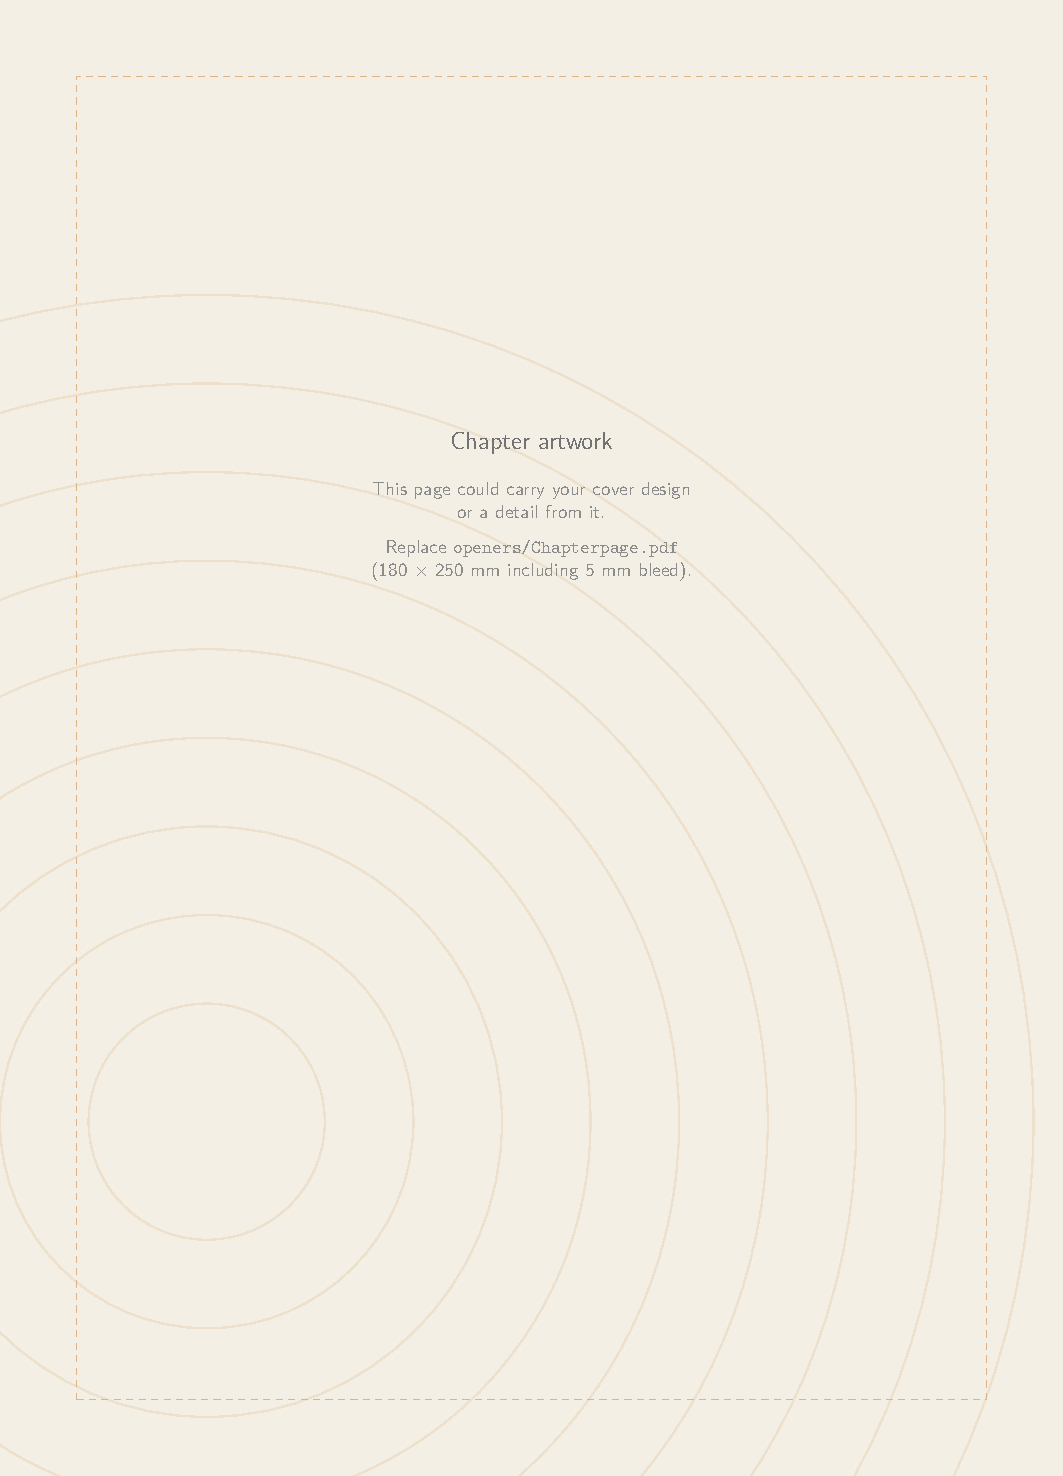
\includegraphics{openers/Chapterpage.pdf}};
      \node[anchor=base,inner sep=0pt,outer sep=0pt,text=chapternumtan]
        at ([xshift=341.58bp+\artbleed,yshift=-550.03bp-\artbleed]current page.north west)
        {\sffamily\fontsize{122bp}{122bp}\selectfont\bfseries #1};
    \end{tikzpicture}%
    \clearpage\nopagecolor\cleardoublepage}{\cleardoublepage}}
\makeatletter
\let\bookorigchapter\chapter
\renewcommand{\chapter}{\@ifstar{\bookorigchapter*}%
  {\ifchapterart\chapterart{\the\numexpr\value{chapter}+1\relax}\fi\bookorigchapter}}
\makeatother
\let\oldappendixart\appendix
\renewcommand{\appendix}{\oldappendixart\chapterartfalse}

